%
%  functions.tex
%  latex_files
%
%  Created by Eyal Shukrun on 08/24/20.
%  Copyright 2020. Eyal Shukrun. All rights reserved.
%
\documentclass{article}
\usepackage[pdftex]{graphicx}
\usepackage[utf8x]{inputenc}
\usepackage{pslatex}
\usepackage{amsmath, amsfonts, amssymb}
\usepackage[hebrew,english]{babel}
\usepackage{cjhebrew}
\usepackage{graphicx}
\graphicspath{ {./images/} }

\title{Fonctions}
\author{Eyal Shukrun}

\begin{document}
\maketitle

Une fonction est définie par trois choses:
\begin{itemize}
  \item Un ensemble de départ
  \item Un ensemble d'arrivée
  \item Une équation
\end{itemize}


\section{Definitions}
\subsection{Ensemble de définition}
Soit $\mathbb{D} = \{1, 2, -2, 4, 5\}$ et $f(x) = x^2$\\
Pour chaque élement $a$ de $\mathbb{D}$ il existe $a^2 \in \mathbb{R}$\\
Ici, $\mathbb{D}$ est considéré comme le \cjRL{t.hwm 'w t.hwm hgdrh} de $f(x)$ (l'ensemble des inputs, ou l'ensemble de départ) et $\mathbb{R}$ est appelé \cjRL{.tww.h} (l'ensemble des outputs, ou ensemble d'arrivée).\\
\subsection{Image}
f(x) est l'image (\cjRL{htmwnh}) de x a travers f.\\
L'ensemble des outputs est l'image de f elle même (par exemple, pour $f(x) = x^2$ définie sur $\{2, -2, 3, 5, 7\}$, 
$\{4, 9, 25, 49\}$ est l'image).\\
L'image d'une fonction est comprise dans son domaine d'arrivée.

\section{Définir une fonction}
\subsection{Grâce à ses domaines de départ et d'arrivée}
On peut définir une fonction en définissant son domaine de départ et les points qui lui correspondent.\\
Par exemple, pour la fonction $f(x) = x^2$ définie sur $\{-2, 2, 3, 4, 5\}$:
\subsubsection{Avec un tableau}
\begin{center}
  \begin{tabular}{ c | c c c c c}
    Départ & -2 & 2 & 3 & 4 & 5\\
    \hline
    Arrivée & 4 & 4 & 9 & 16 & 25
 \end{tabular}
\end{center} 

\subsubsection{Avec des couples ordonnés}
Le premier chiffre du couple correspond a l'input et le deuxième a l'output:\\
\begin{center}
$f = \{(-2,4), (2,4), (3,9), (4,16), (5,25) \}$
\end{center}
\textbf{Remarque:} On note ce groupe $f$ car il represente la fonction $f$.\\
\textbf{Remarque:} Si une fonction f est définie de $\mathbb{D}$ a $T$ ($f : D \to T$), et que $S$ est un sous ensemble de $\mathbb{D}$ ($S \subseteq D$), alors l'image de $S$ par $f$ est écrite $f(S)$. $f(S)$ contient toutes les images des éléments de $S$ par $f$.\\
\textbf{Attention:} Pour qu'un ensemble de groupes ordonnés soit representatif d'une fonction, il est impératif de ne pas trouver deux tuples avec le meme premier élement.

\subsection{Avec une équation}
Pour définir une fonction, une équation n'est pas suffisante, il faut aussi préciser son domaine de définition.\\
\begin{align*}
  &f : Z \to Z\\
  &f(x) = x^2 + 7x - 15
\end{align*}
  
\section{Fonctions bijectives, surjectives et injectives}
\begin{center}
  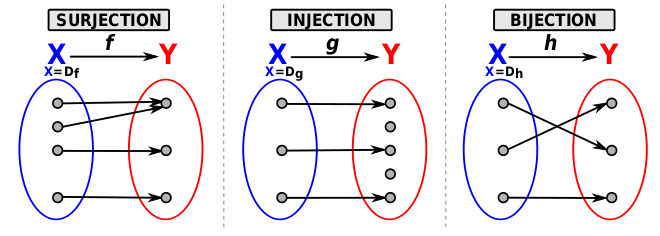
\includegraphics[scale=0.5]{surjection_injection_bijection}
\end{center}

\subsection{Fonctions bijectives}
  
Une fonction bijective (\cjRL{pwnq.syh .hd .hd `rkyt}) est une fonction qui n'a qu'un seul input par output.\\

\subsection{Fonctions surjectives}
Une fonction surjective est une fonction pour laquelle chaque élément de l'ensemble d'arrivée est l'image d'au moins un élément de l'ensemble de départ, cela implique que $f: A \to B \Rightarrow f(A) = B$
 
\section{Démonstrations}
\subsection{Prouver qu'une fonction est bijective}
Pour prouver qu'une fonction est bijective, il suffit de prouver que:
\begin{align*}
  f(a) = f(b) \Rightarrow a = b
\end{align*}

\subsection{Prouver que l'image d'une fonction appartient a un ensemble}
Soit:
\begin{align*}
  &f : R \to R\\
  &f(x) = \frac{1}{2}x - \frac{1}{2}
\end{align*}
Prouver que $f(R) = R$:\\
\\
\textbf{1. Prouver que $f(R) \subseteq R$, il n'y a rien a prouver.\\}
\textbf{2. Prouver que $R \subseteq f(R)$:\\}
Soit $y \in R$, prouvons que $y \in f(R)$\\
C'est a dire prouvons qu'il existe $x \in R$ tel que $f(x) \in R$.\\
C'est a dire prouvons qu'il existe pour tout $x \in R$ $f(x) = y$
\begin{align*}
  x &= 2(y + \frac{1}{2})\\
  x &= 2y + 1\\
  f(x) &= f(2y +1)\\
  f(2y + 1) &= \frac{1}{2}(2y + 1) - \frac{1}{2}\\
  f(2y + 1) &= y+\frac{1}{2} - \frac{1}{2} \\
  f(2y + 1) &= y\\
\end{align*}

\section{Composition de fonctions}
Soit une fonction $f$ et une fonction $g$, tel que l'ensemble d'arrivée de $f$ est compris dans l'ensemble de départ de $g$. Il existe donc une nouvelle fonction $g(f(x))$, qui est une composition de $f$ et $g$, notée $g \circ f$.\\
\textbf{Remarque}: $g \circ f$ n'est pas pareil que $f \circ g$, l'ordre compte (l'input rentre dans la fonction la plus a droite d'abord).

\section{Fonctions inverses}
Soit $f$ une fonction bijective (pour chaque output, il n'existe qu'un seul input), existe t'il une fonction permettant de passer d'une output a l'input qui lui correspond ? \\
C'est le principe de la fonction inverse (\cjRL{pwnq.syh hpwkh}), notée $f^{-1}$.\\
Ainsi, $f(x) = y \Leftrightarrow f^{-1}(y) = x$\\
On peut aussi dire que $f^{-1} = \{(y,x) | (x,y) \in F\}$\\

\subsection{Fonction identité}
Une fonction identité (\cjRL{pwnq.syt zhwt}) est une fonction dont chaque input est son propre output.\\
Ainsi, la fonction $f^{-1} \circ f$ est une fonction identité.\\ 
\textbf{Remarque}: Pour tout $f : S \to D$, $f^{-1} \circ f = I_{S}$ ($I_{S}$ est la fonction identi)
       
  
\end{document}
